\documentclass[journal]{new-aiaa}
%\documentclass[conf]{new-aiaa} for conference papers
\usepackage[utf8]{inputenc}
\usepackage{textcomp}

\usepackage{graphicx}
\usepackage{amsmath}
\usepackage[version=4]{mhchem}
\usepackage{siunitx}
\usepackage{longtable,tabularx}
\usepackage{multicol}
\usepackage{geometry} % For custom page size and margins
\setlength\LTleft{0pt} 

% Set custom page size and margins for a total width of 7 inches
\geometry{
  letterpaper, 
  left=0.375in, 
  right=0.375in, 
  top=1in, 
  bottom=1in, 
  columnsep=0.5in % Space between the two columns
}


\title{Thermo-mechanical Impact of Thruster Plume Impingement on Space Debris}

\author{Jacob Higgins \footnote{Undergraduate Student, School of Civil, Aerospace, and Design Engineering, jacob.higgins.2021@bristol.ac.uk.} and Lucy Berthoud \footnote{Professor, School of Civil, Aerospace, and Design Engineering.}}
\affil{University of Bristol Queen's Building, BS8 2TR, United Kingdom}

\begin{document}
\onecolumn
\maketitle

\begin{abstract}
Active debris removal (ADR) is defined as a capability to interact with passive orbiting objects, in order to reduce their orbital lifetime \cite{steeringgroupIADCStatementActive2022a}. It is known that ADR is necessary to control the unstable growth rate of debris in low Earth orbit (LEO)\cite{inter-agencyspacedebriscoordinationcommitteePeacefulUsesOuter1993} \cite{bastidavirgiliActiveDebrisRemoval2013}. Considerable work hads been done on assessing the feasiblity of active debris removal missions (cite lots here). One proposed method for this is to use plume impinegement of a reaction control system (RCS) thruster on the capturing spacecraft. This work looks at the effect of the mechanical and thermal effcts of a thruster plume on the debris, in order to assess the risk that this detumbling method could cause break-off of material and appendages such as solar panels and antennas. A classification of the severity of different potential debris objects is also presented, in order to quantify this risk of this method, in terms of the likelihood of break-off and the potential impact of the debris.
\end{abstract}


\section*{Nomenclature}

\noindent(Nomenclature entries should have the units identified)

{\renewcommand\arraystretch{1.0}
\noindent\begin{longtable*}{@{}l @{\quad=\quad} l@{}}
$\rho$ & density\\
$p$ & pressure \\
$m$ & mass\\
$T$ & Temperature\\
$\sigma_T$ & collision cross section\\
$\Theta$ & boundary-layer momentum thickness\\
\multicolumn{2}{@{}l}{Subscripts}\\
$E$ & Nozzle exit flow conditions \\
$*$ & Throat flow conditions \\
$0$ & Stagnation flow conditions \\
\end{longtable*}}

\twocolumn
\section{Introduction}
\label{sec-introduction}


Active debris removal (ADR) is defined as a capability to interact with passive orbiting objects, in order to reduce their orbital lifetime \cite{steeringgroupIADCStatementActive2022a}. It is known that ADR is necessary to control the unstable growth rate of debris in low Earth orbit (LEO) \cite{inter-agencyspacedebriscoordinationcommitteePeacefulUsesOuter1993} \cite{bastidavirgiliActiveDebrisRemoval2013}. Considerable work hads been done on assessing the feasiblity of active debris removal missions \cite{ledkovReviewContactContactless2022,bonnalActiveDebrisRemoval2013}. It showed that during ADR, it is necessary to minimise the different in spin rates between debris and the capturing spacecraft \cite{shanReviewComparisonActive2016}. One proposed method of de-tumbling is to use plume impinegement of a reaction control system (RCS) thruster on the capturing spacecraft, to create a moment on the debris \cite{peters2016applicability,ferrariGASPLUMEIMPINGEMENT2014}. 

\subsection{Plume Impingement}

A thruster plume in space expands differently to in atmosphere, due to the severely low downstream pressure in vacuum. Expansion fans at the nozzle exit do not expand according to the Prandtl-Mayer angle, but instead expand more radially as if eminating from a point source at the centre of the nozzle \cite{mehtaUnderexpandedSupersonicPlume2011}. The low downstream pressure also leads to a decreasing mean free path in the plume. Mean free path is the average distance travelled by a particle between successive particular collisions:

\begin{equation}
  \lambda = \frac{m}{\sqrt{2} \rho {\sigma}_T} 
  \label{intro_eq_meanFreePath}
\end{equation}

As $\lambda$ increases, the gas transitions from behaving like a continuum where Navier-Stokes (and all derived flow equations) are valid, to a rarefied gas where instead kinetic theory must be applied to accurately capture the particular nature of the gas \cite{pittPlumeImpingementStudies}. The Knudsen number is commonly used to quantify the transition from continuum to rarefaction \cite{knudsenGesetzeMolekularstromungUnd2006}. This parameter is equal to the mean free path, normalised by a characteristic length. In literature for plume impingement studies, the characteristic length chosen is commonly a nozzle parameter, but can differ between nozzle radius, nozzle diameter, throat radius, and nozzle length \cite{caiGaskineticSolutionsHigh2013,sharmaDSMCSimulationRocket2023,singhalNumericalStudyNozzle2024,subramanianUnderexpandedJetImpingement2024}. Knudsen number is used to split the plume into three regions: continuum region; transition region; and the free molecular region. These regions and the applicable Knudsen number ranges are shown in Figure \ref{intro_fig_FlowRegions}. In the transition region, the gas is nether a continuum or rarefied gas. Often, direct simulation monte carlo (DSMC) computations are used to characterise this region of the flow. In addition, DSMC codes allow for the computation of non-equilibrium thermal balance conditions between a plume and the surface upon which it impinges. Notably, when running DSMC calculations, the distiction between the flow regions from Figure \ref{intro_fig_FlowRegions} is generally determined by Bird's parameter rather than the Knudsen number. Bird's parameter is simply the Knudsen number where the characteristic length is constrained to the cell size of the mesh \cite{birdMolecularGasDynamics2003}. Legge had some success by omitting the transition region, and treating the flow as either continuum or rarefied \cite{leggeModellingControlThruster1982}. Impingement was then calculated in the transition regime by estimating a reduced pressure coefficient: an average of pressure coeffients in the adjacent continuum and free molecular regions. In Legge's case, this averaging was based on experimental data of his specific thruster, and so likely does not constitute a valid general method.




\begin{figure}[ht]
  \centering
  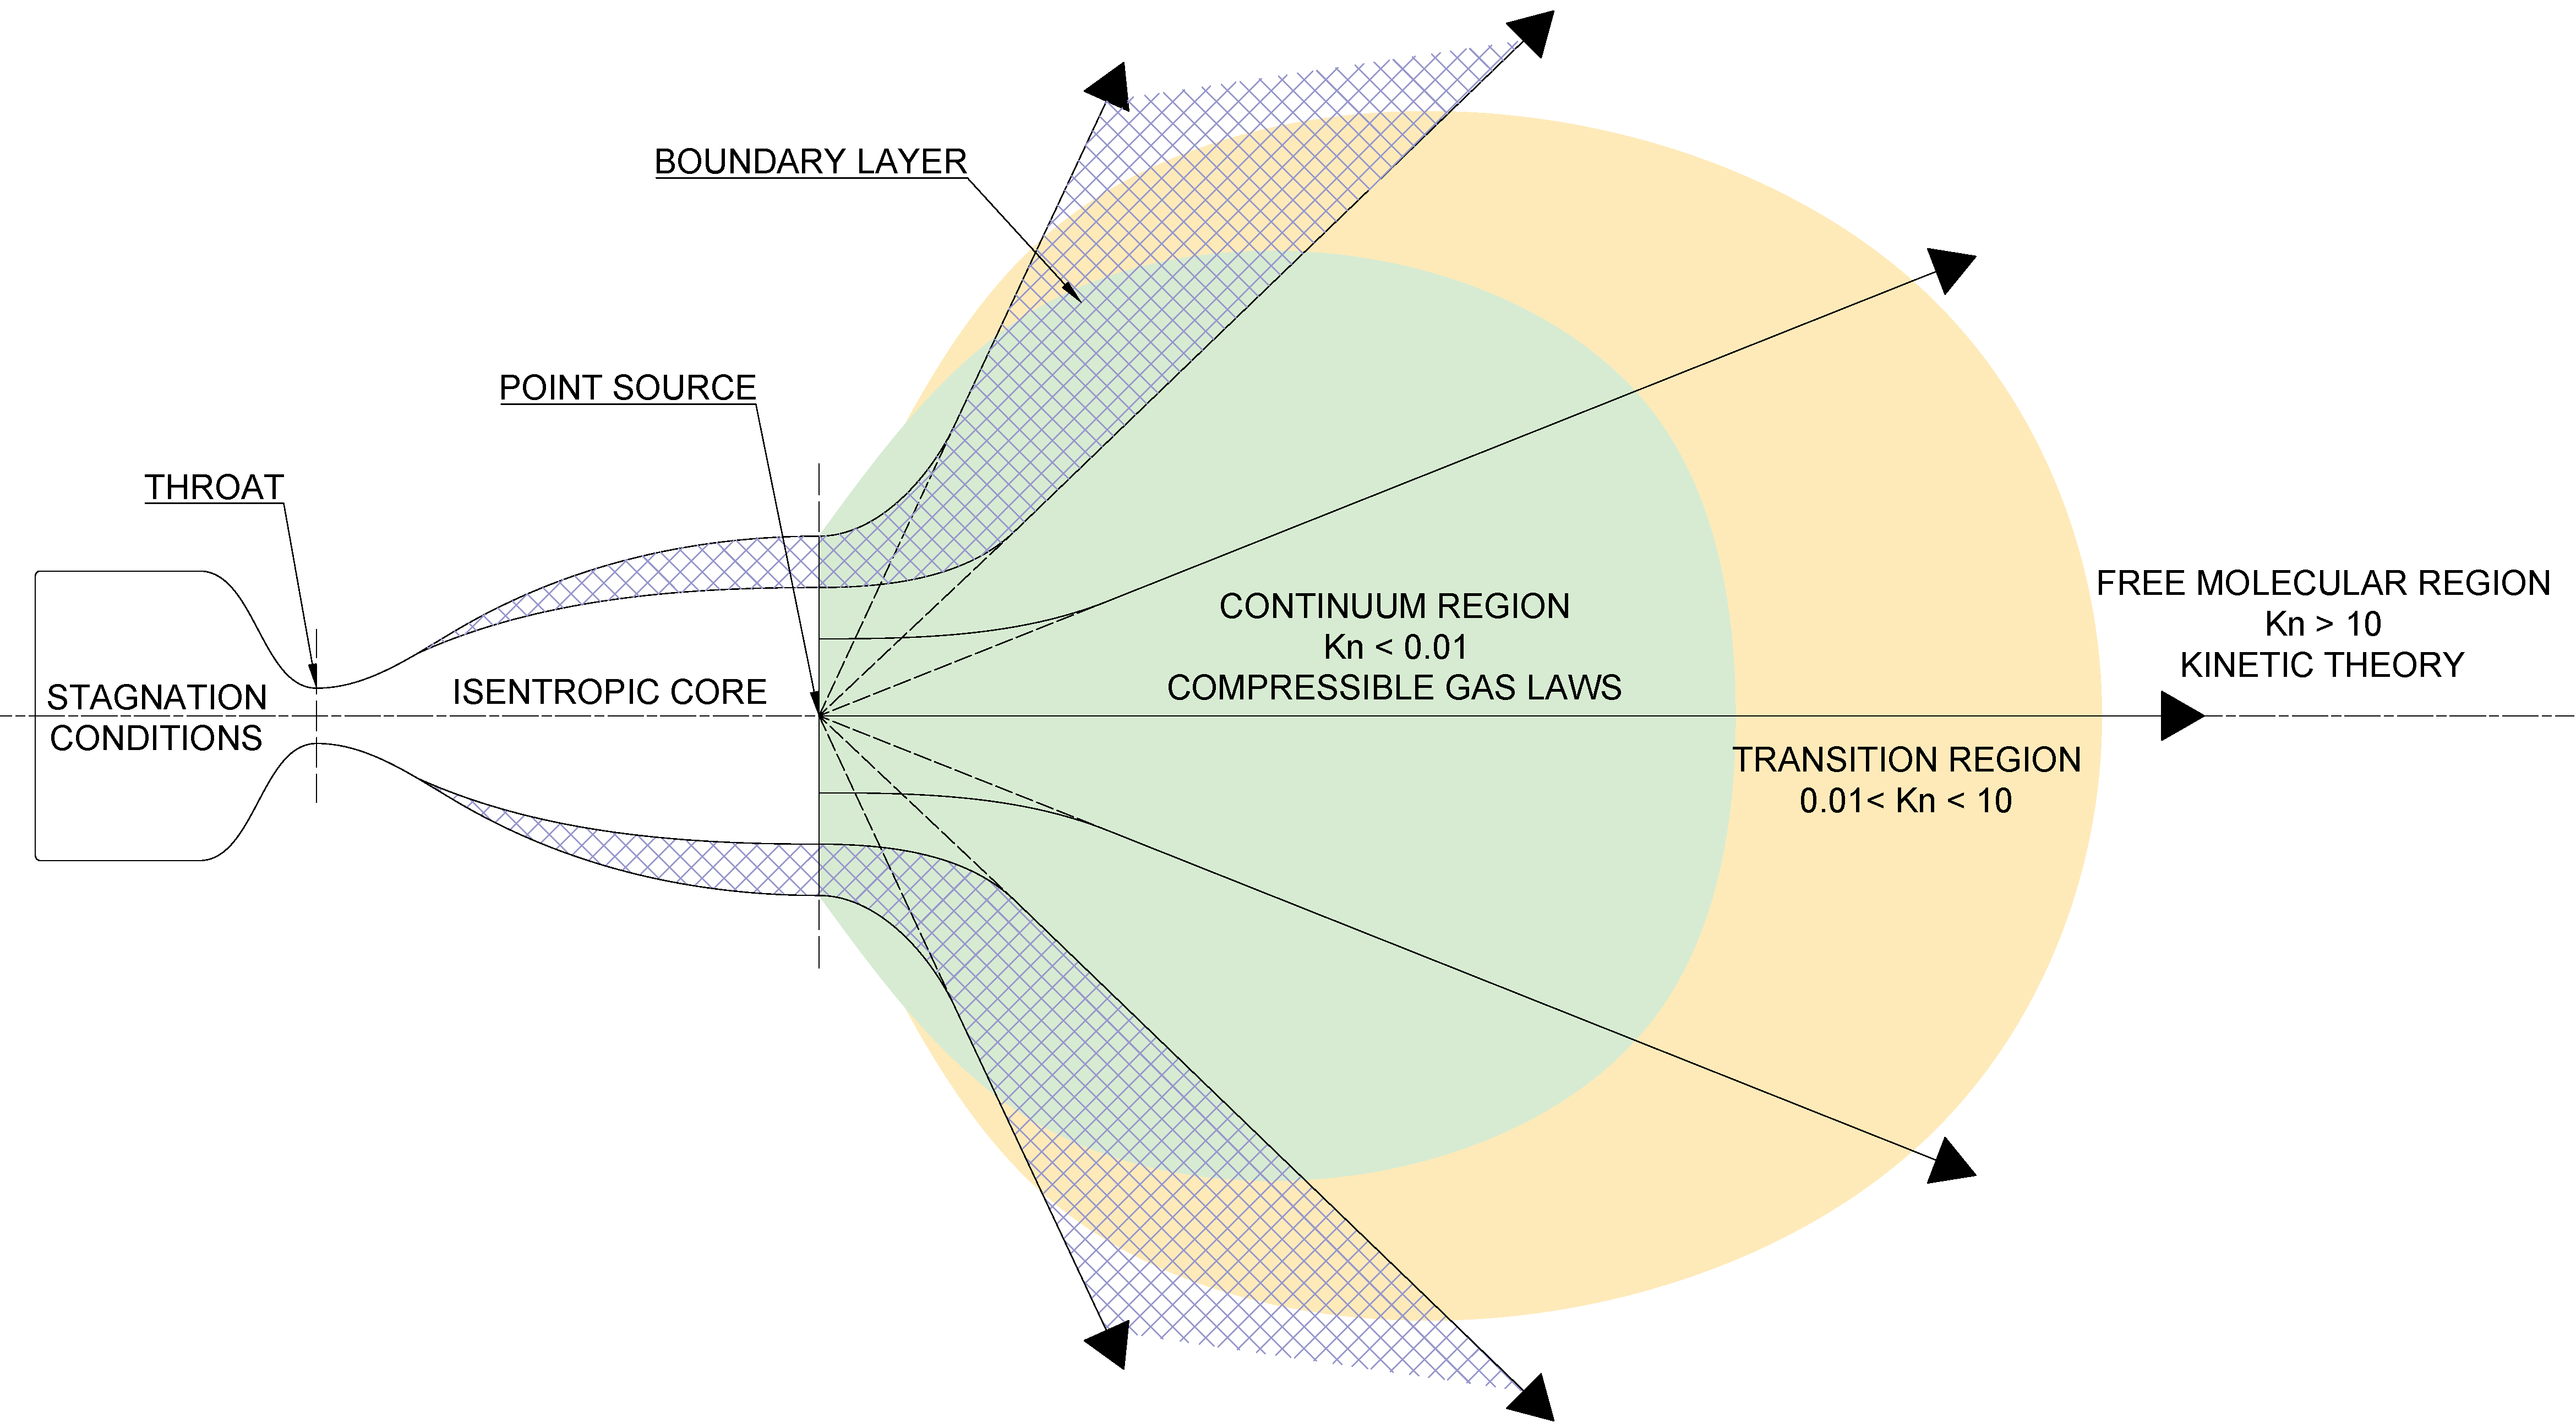
\includegraphics[width=\columnwidth]{Figures/FlowRegions.pdf}
  \caption{Flow Regions from an isentropic nozzle exhaust, and their characteristic Knudsen number ranges.}
  \label{intro_fig_FlowRegions}
\end{figure}

Equation \ref{intro_eq_meanFreePath} shows for a plume with a single particle species A, and hence a constant particular mass and collision cross section, the mean free path is inversly proportional to the density of the plume. Analytical methods for determining the density field of the plume commonly include Simon's model and Mayer's model \cite{simonsEffectNozzleBoundary1972} \cite{mayerThrustLossDue1986}. Both of these models estimate the density to decay with axial distance from the nozzle exit, and angle from the centreline. The methods estimate the plume based on the boundary layer thickness of the (assumed isentropic) nozzle flow. Hence, it is critical that the nozzle exit conditions are well defined, ideally by experimental data. It has also been shown that these methods are only valid in the continuum region of the plume \cite{boydModelingSmallHydrazine1990}.

When a plume comes into contact with a surface, it impinges some of the plume energy onto the surface- causing temperature increases and forces on the surface. The impingement of the plume onto a surface is found by imagining a freezing plane. Importantly, analytical models assume that the presence of the surface has no effect on the plume shape and properties; hence the impinged flux and pressure is independent of the freezing surface geometry \cite{herraiz2019development}. From flux and pressure, the temperature of the surface and the force imparted in it can be found from standard equations. Ultimately, it can be determinded whether the imparted force will cause failure of the surface at the elevated temperature. Since the impinged surface is debris, and has therefore likely been on-orbit for considerable time, the degredation of the materials due to the space environment (radiation, UV exposure) must also be accounted for when determinng the mechanical properties of the surface.



%END OF PLUME IMPINGEMENT SECTION 
\subsection{Debris Risk from ThermoMechanical Effect}

DISCUSSION OF DEBRIS SEVERITY EVALUATION METHODS
AND THERMAL AND MECHANICAL 'PROBLEMS' ON THE DEBRIS


The severity of any potential debris created must also be assessed. This serverity is most closely associated with the momentum of the debris, and hence the mass. However, the hardness of the debries can also be considered, as a good indicator to the potential sharpness of any debris created. The mass of induvidual debris object may be considered in larger cases, but in cases of multiple smaller breakeages, it is the mass of the debris cloud that must be considered. 



I also need to talk hear about the thermal effect of a plume. That is that heat flux can cause melting. Melting of glue between composites, meting of glue for attatchments. 


This work looks at the mechanical and thermal effcts of a thruster plume on the debris, in order to assess the risk that this detumbling method could cause break-off of material and appendages, such as solar panels and antennas. A classification of the severity of different potential debris objects is also presented, in order to quantify the risk of this method in terms of the likelihood of break-off and the potential impact of the debris.




\section{Methodology}
\label{sec-methodolody}



\section*{Appendix}

An Appendix, if needed, appears \textbf{before} research funding information and other acknowledgments.

\section*{Funding Sources}

Sponsorship information and acknowledgments of financial support should be included here. \textbf{Authors are responsible for accurately reporting funding data relevant to their research.} Please confirm that you have correctly entered \textbf{all sources} of funding and grant/award numbers \textbf{for all authors} in this section of your article. You will also be asked to select the appropriate funding organization from a drop-down menu in ScholarOne when you submit your manuscript. Be careful to choose the correct funder name, as organization names can be similar, and also be mindful to select sub-organizations within the registry hierarchy that are the actual funding sources, as appropriate, rather than choosing the name of the parent organization. Information provided in your manuscript must match the funding data entered in ScholarOne.

\section*{Acknowledgments}
An Acknowledgments section, if used, \textbf{immediately precedes} the References. Individuals other than the authors who contributed to the underlying research may be acknowledged in this section. The use of special facilities and other resources also may be acknowledged. 


\bibliography{references.bib}

\end{document}
